\section{Just-In-Time Compiler}
\begin{itemize}
    \item Effizientere Ausführung als Interpretation
    \item Bytecode direkt in nativen Prozessor-Code übersetzen und ausführen
    \item Nicht unbedingt alles, sondern nur kritische Teile
\end{itemize}

\subsection{Hot Spot}
\begin{itemize}
    \item Performance-kritisher Code Abschnitt
    \item Wird häufig ausgeführt
    \item JIT-Kompilierung loht sich hierfür am meisten
\end{itemize}

\subsection{Profiling}
\begin{itemize}
    \item Interpreter zählt Ausführung gewisser Code-Teile (Methoden, Traces (Code-Pfade))
    \item Falls häufig ausgeführt, JIT für den Teil anwerfen
\end{itemize}

\subsection{Vorgehen}
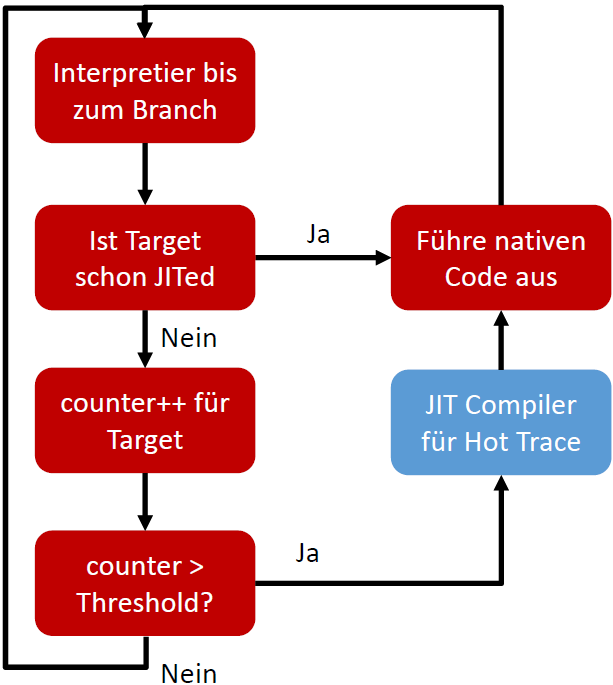
\includegraphics[width=0.4\linewidth]{jit_vorgehen.png}

\subsection{Intel 64 Architektur}
\textbf{Spezielle Register}
\begin{itemize}
    \item RSP: Stack Pointer
    \item RBP: Base Pointer
    \item RIP: Instruction Pointer
\end{itemize}
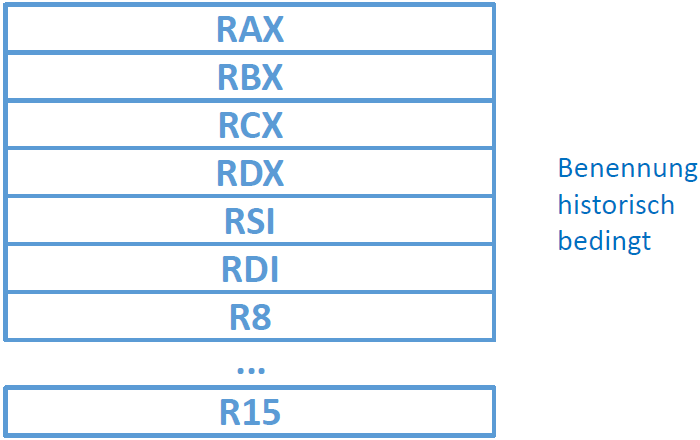
\includegraphics[width=0.5\linewidth]{intel1.png}
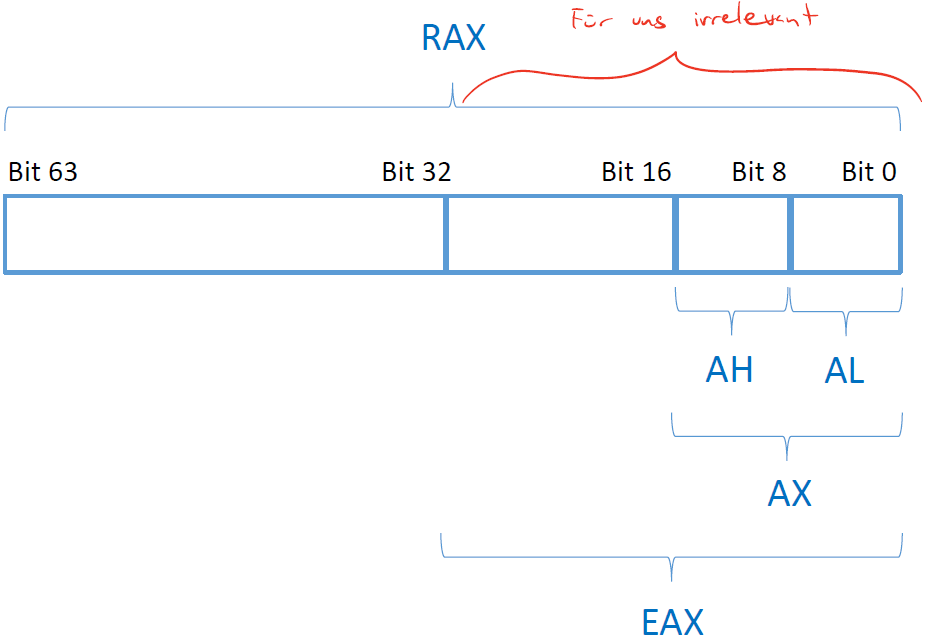
\includegraphics[width=0.5\linewidth]{intel2.png}

\subsubsection{Elementare Instruktionen}
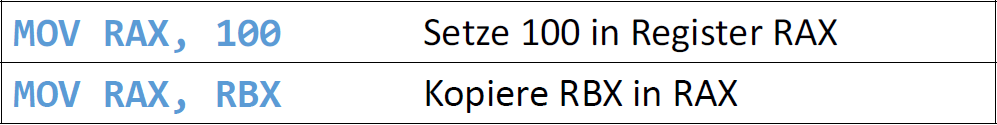
\includegraphics[width=0.5\linewidth]{elementare_instruktionen.png}
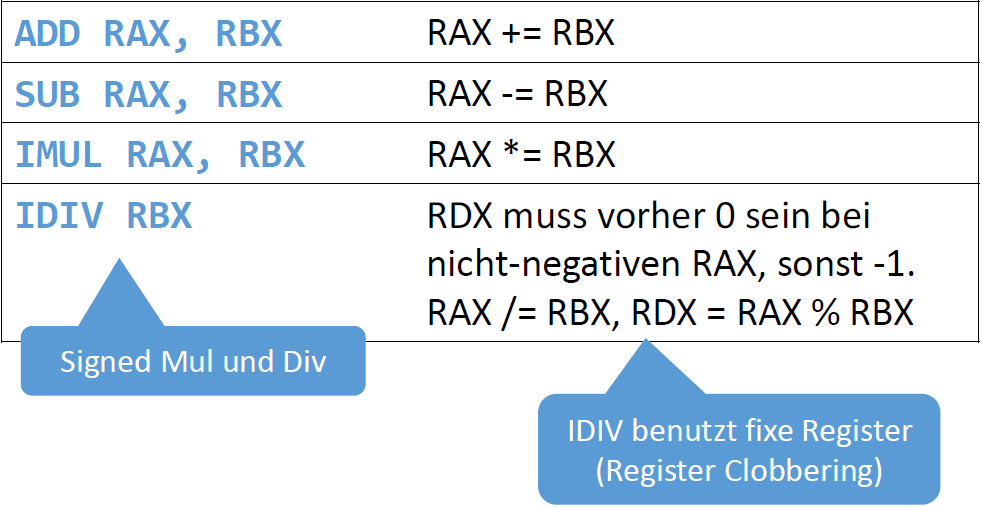
\includegraphics[width=0.5\linewidth]{arithm_instruktionen.png}

\subsubsection{IDIV Vorbereiten}
\begin{itemize}
    \item Fixe 128-bit Division von RDX:RAX
    \item Setze RDX je nach RAX
    \begin{itemize}
        \item 0 falls RAX $>=$ 0
        \item -1 falls RAX $<$ 0
    \end{itemize}
\end{itemize}
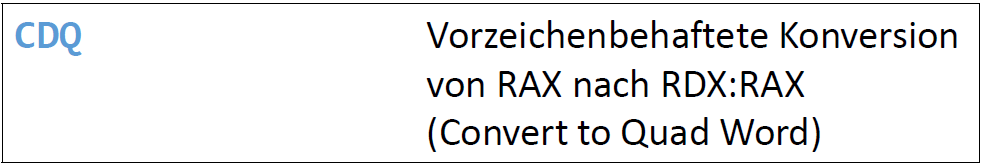
\includegraphics[width=0.5\linewidth]{cdq.png}

\subsection{Register Allokation}
\textbf{Lokale Register Allokation}
\begin{itemize}
    \item Für Ausdrucksauswertung (Evaluation Stack)
    \item Evaluation Stack Einträge auf Register abbilden
    \item Cross Compiler führt Stack an belegten Register 
    \item Pro übersetzte Bytecode-Instruktion wird Stack nachgeführt
\end{itemize}
\textbf{Globale Register-Allokation}
\begin{itemize}
    \item Veriablen in Register speichern
    \item Deutlich schneller als Speicherzugriffe
    \item Parameter werden oft als Register übergeben (Calling Convention)
\end{itemize}
\textbf{Registeranzahl ist beschränkt!}

\subsection{Register Clobbering}
\begin{itemize}
    \item Evakuiere in neues Register bei Instruktionen mit fixem Operand (z.B. IDIV)
\end{itemize}
\subsubsection{Register Relocation}
\begin{itemize}
    \item Umkopieren in anderes Register
\end{itemize}
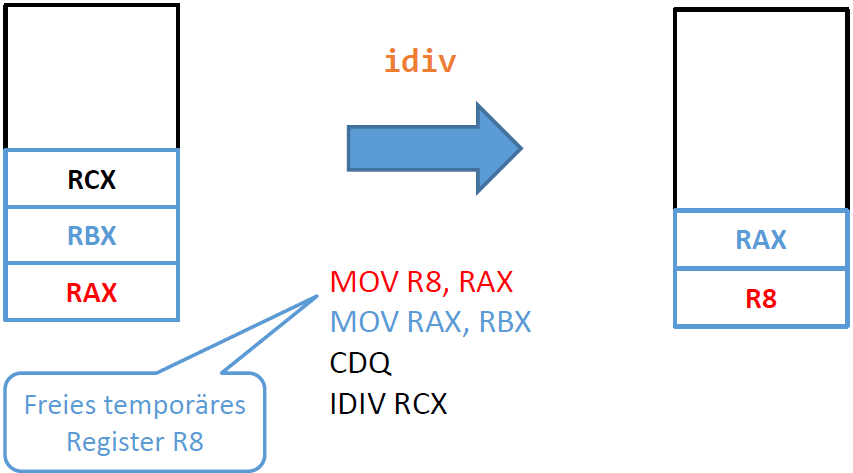
\includegraphics[width=0.5\linewidth]{register_relocation.png}

\subsection{Intel Branches}
\begin{itemize}
    \item Bedingte Sprünge basierend auf Condition Code
    \item Condition Code aus vorherigem Vergleich
\end{itemize}
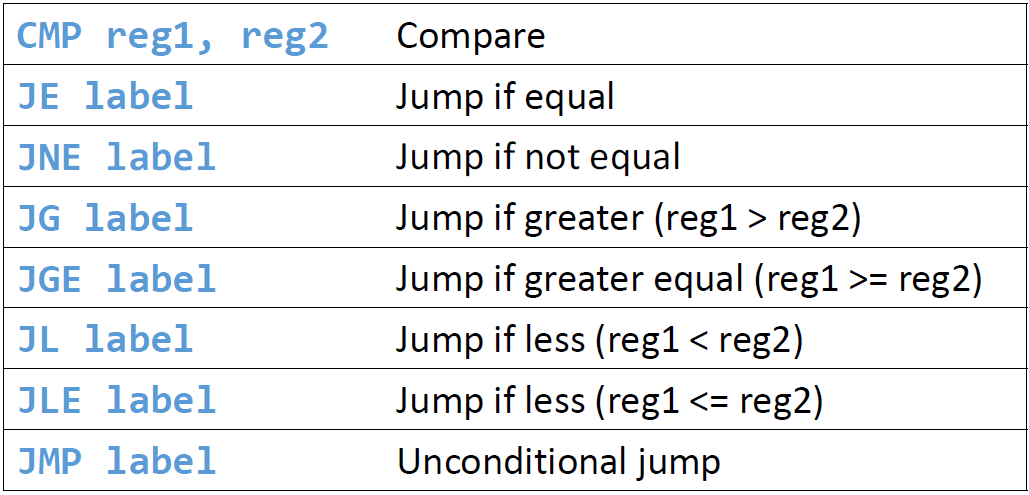
\includegraphics[width=0.5\linewidth]{branch_instruktionen_intel.png}
